\documentclass[border=1pt]{standalone}
\usepackage{tikz}
\usepackage[compat=1.0.0]{tikz-feynman}
\usepackage{contour}

\begin{document}
\begin{tikzpicture}
  \begin{feynman}
    \vertex (s1) at (-.6,0);
    \vertex (s2) at (.6, 0);
    \vertex (a) at (-2, 1) {\(q\) };
    \vertex (b) at (-2,-1) {\(\bar{q}\) };
    \vertex (c) at ( 2, 1) {\(\bar{\chi}\)};
    \vertex (d) at ( 2,-1) {\(\chi\)};

    \diagram[layered layout, horizontal=s1 to s2] {
      (a) -- [fermion] (s1) -- [fermion] (b),
      s1 -- [scalar, edge label'=\(S\)] (s2)
      (c) -- [fermion] (s2) -- [fermion] (d),
    };
  \end{feynman}
\end{tikzpicture}

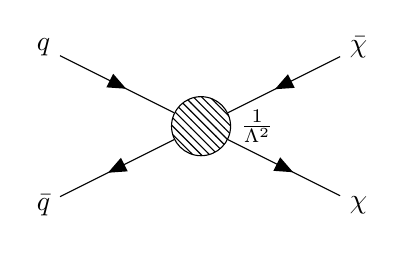
\begin{tikzpicture}
  \begin{feynman}
    \vertex[blob, label={right: $\frac{1}{\Lambda^{2}}$}] (m) at (0, 0){};
    \vertex (a) at (-2, 1) {\(q\) };
    \vertex (b) at (-2,-1) {\(\bar{q}\) };
    \vertex (c) at ( 2, 1) {\(\bar{\chi}\)};
    \vertex (d) at ( 2,-1) {\(\chi\)};
    \diagram* {
      (a) -- [fermion] (m) -- [fermion] (b),
      (c) -- [fermion] (m) -- [fermion] (d),
    };
  \end{feynman}
\end{tikzpicture}
\end{document}
